\documentclass[conference]{IEEEtran}

\usepackage{cite}
\usepackage{amsmath,amssymb,amsfonts}
\usepackage{verbatim} % um viele zeilen auszukommentieren
\usepackage{algorithmic}
\usepackage{graphicx}
\usepackage[ngerman]{babel}		% Achtung umlaut 
\usepackage[utf8]{inputenc}       % UTF-8 ist wichtig,  ASCII hat nicht alle Schriftzeichen  
\usepackage{textcomp}
\usepackage{xcolor}
\usepackage{dirtytalk} % nein, nicht was du denkst.  Packet hilft  gegen verschluckte gänsefüschen
\def\BibTeX{{\rm B\kern-.05em{\sc i\kern-.025em b}\kern-.08em
    T\kern-.1667em\lower.7ex\hbox{E}\kern-.125emX}}
\begin{document}

\title{Projekt rosBerry *\\
{\footnotesize \textsuperscript{*}Ein Autonomer Roboter auf der Basis von ROS , gebaut aus einem Modeauto Chassis mit Maker Elektronik}}

\author{\IEEEauthorblockN{1\textsuperscript{st} Welter, Heike}
\IEEEauthorblockA{\textit{Hochschule Mannheim} \\
email address 1630298@stud.hs-mannheim.de}%
\and
\IEEEauthorblockN{2\textsuperscript{nd} Matteis, Steffen}
\IEEEauthorblockA{\textit{Hochschule Mannheim} \\
email address}%noch 
\and
\IEEEauthorblockN{3\textsuperscript{rd}Barsalou Marie }
\IEEEauthorblockA{\textit{Hochschule Mannheim} \\
email address}
}

\maketitle

\begin{abstract}
Ziel von rosBerry besteht darin einen kleinen, schnellen aber dennoch preisgünstigen Roboter aus leicht verfügbaren Standartbauteilen zu Bauen. rosBerry unterscheidet sich durch die Verwendung von ROS und KI Techniken von dem DonkeyCar Projekt
\end{abstract}

\begin{IEEEkeywords}
Roboter, ROS, KI, Raspi, Neuronale Netze, Arduiono
\end{IEEEkeywords}

%\section{Einleitung }  wollen wir  eine machen?
%projekteinleitung text hier
\section{Theorie zu dem Roboter und seiner Künstlichen Intelligenz}

\subsection{Vergleichbare Projekte}	%mary
Wenige Projekt der Robotik oder der Künstlichen Intelligenz für Autonome Systeme  existieren ohne das es nicht andere Vergleichbare Projekte gibt. \\
Die Hardware des Roboters wurde vom Donkey car Projekt inspieriert. Das Neuronale Netz zur Bildklassifizierung ist an das Buch  Artificial Intelligence for Robotics  \cite{b1} angelehnt. 

\subsubsection{Vergleichbare Hardware Ansätze Donkey Cars} %may
%Donkey car infos
https://docs.donkeycar.com
% Tiziano der Rasende Italiener auf youtube
\subsubsection{Vergleichbare Projekte zur Künstlichen Intelligenz} %steffen ? mary?
%buch as dem wir das KI tutorial haben
\subsection{Neuronale Netze in Theorie}	%steffen

\subsubsection{Ansätze für die Erstellung vom Datensatz}	%mary
% wiso das marker symbol
% bilder ++
% wie unterschiedliche bilder

\section{Praktische Projekt Durchführung }

\subsection{Hardware aufbau}%Heike 

\subsection{Grobübersicht über das System}	%heike

\subsection{ROS Knoten Software Architektu}

\subsubsection{ Launch Reihenfolge}%heike

\section{Autonomes verhalten durch Künstliche Intelligenz  }	%mary
%was machen wir da eigentlich
%was ist unser ziel
%wiso haben wir uns dafür entschiden

\subsection{Erster Ansatz für das Neuronale Netz}	%steffen ? mary?
%netzaufbau am anfang
\subsubsection{Este Auswertung der Ergebnisse}	%steffen? 
%wiso war das scheisse
\subsection{Schritte zur Verbesserungen der Erkennungsrate} %mary
%was haben wir dann gemacht 
\subsection{Anwendung des Trainingsmodells } %steffen +mary
%bild teilen
%bild analysieren
%  entscheidung treffen, rechts, links geradeaus oder rückwärtz
\subsection {Auswertung des verhalten des Roboters}
%macht er irgendwas sinnvolles? ist er klüger als eine eintagsfliege

\begin{comment}	%  how-to formeln 
\begin{equation}
a+b=\gamma\label{eq}
\end{equation}
\end{comment}
\begin{comment}
\paragraph{Positioning Figures and Tables} 
 Use the abbreviation 
``Fig.~\ref{fig}'', even at the beginning of a sentence.

\begin{table}[htbp]
\caption{Table Type Styles}
\begin{center}
\begin{tabular}{|c|c|c|c|}
\hline
\textbf{Table}&\multicolumn{3}{|c|}{\textbf{Table Column Head}} \\
\cline{2-4} 
\textbf{Head} & \textbf{\textit{Table column subhead}}& \textbf{\textit{Subhead}}& \textbf{\textit{Subhead}} \\
\hline
copy& More table copy$^{\mathrm{a}}$& &  \\
\hline
\multicolumn{4}{l}{$^{\mathrm{a}}$Sample of a Table footnote.}
\end{tabular}
\label{tab1}
\end{center}
\end{table}

\begin{figure}[htbp]
\centerline{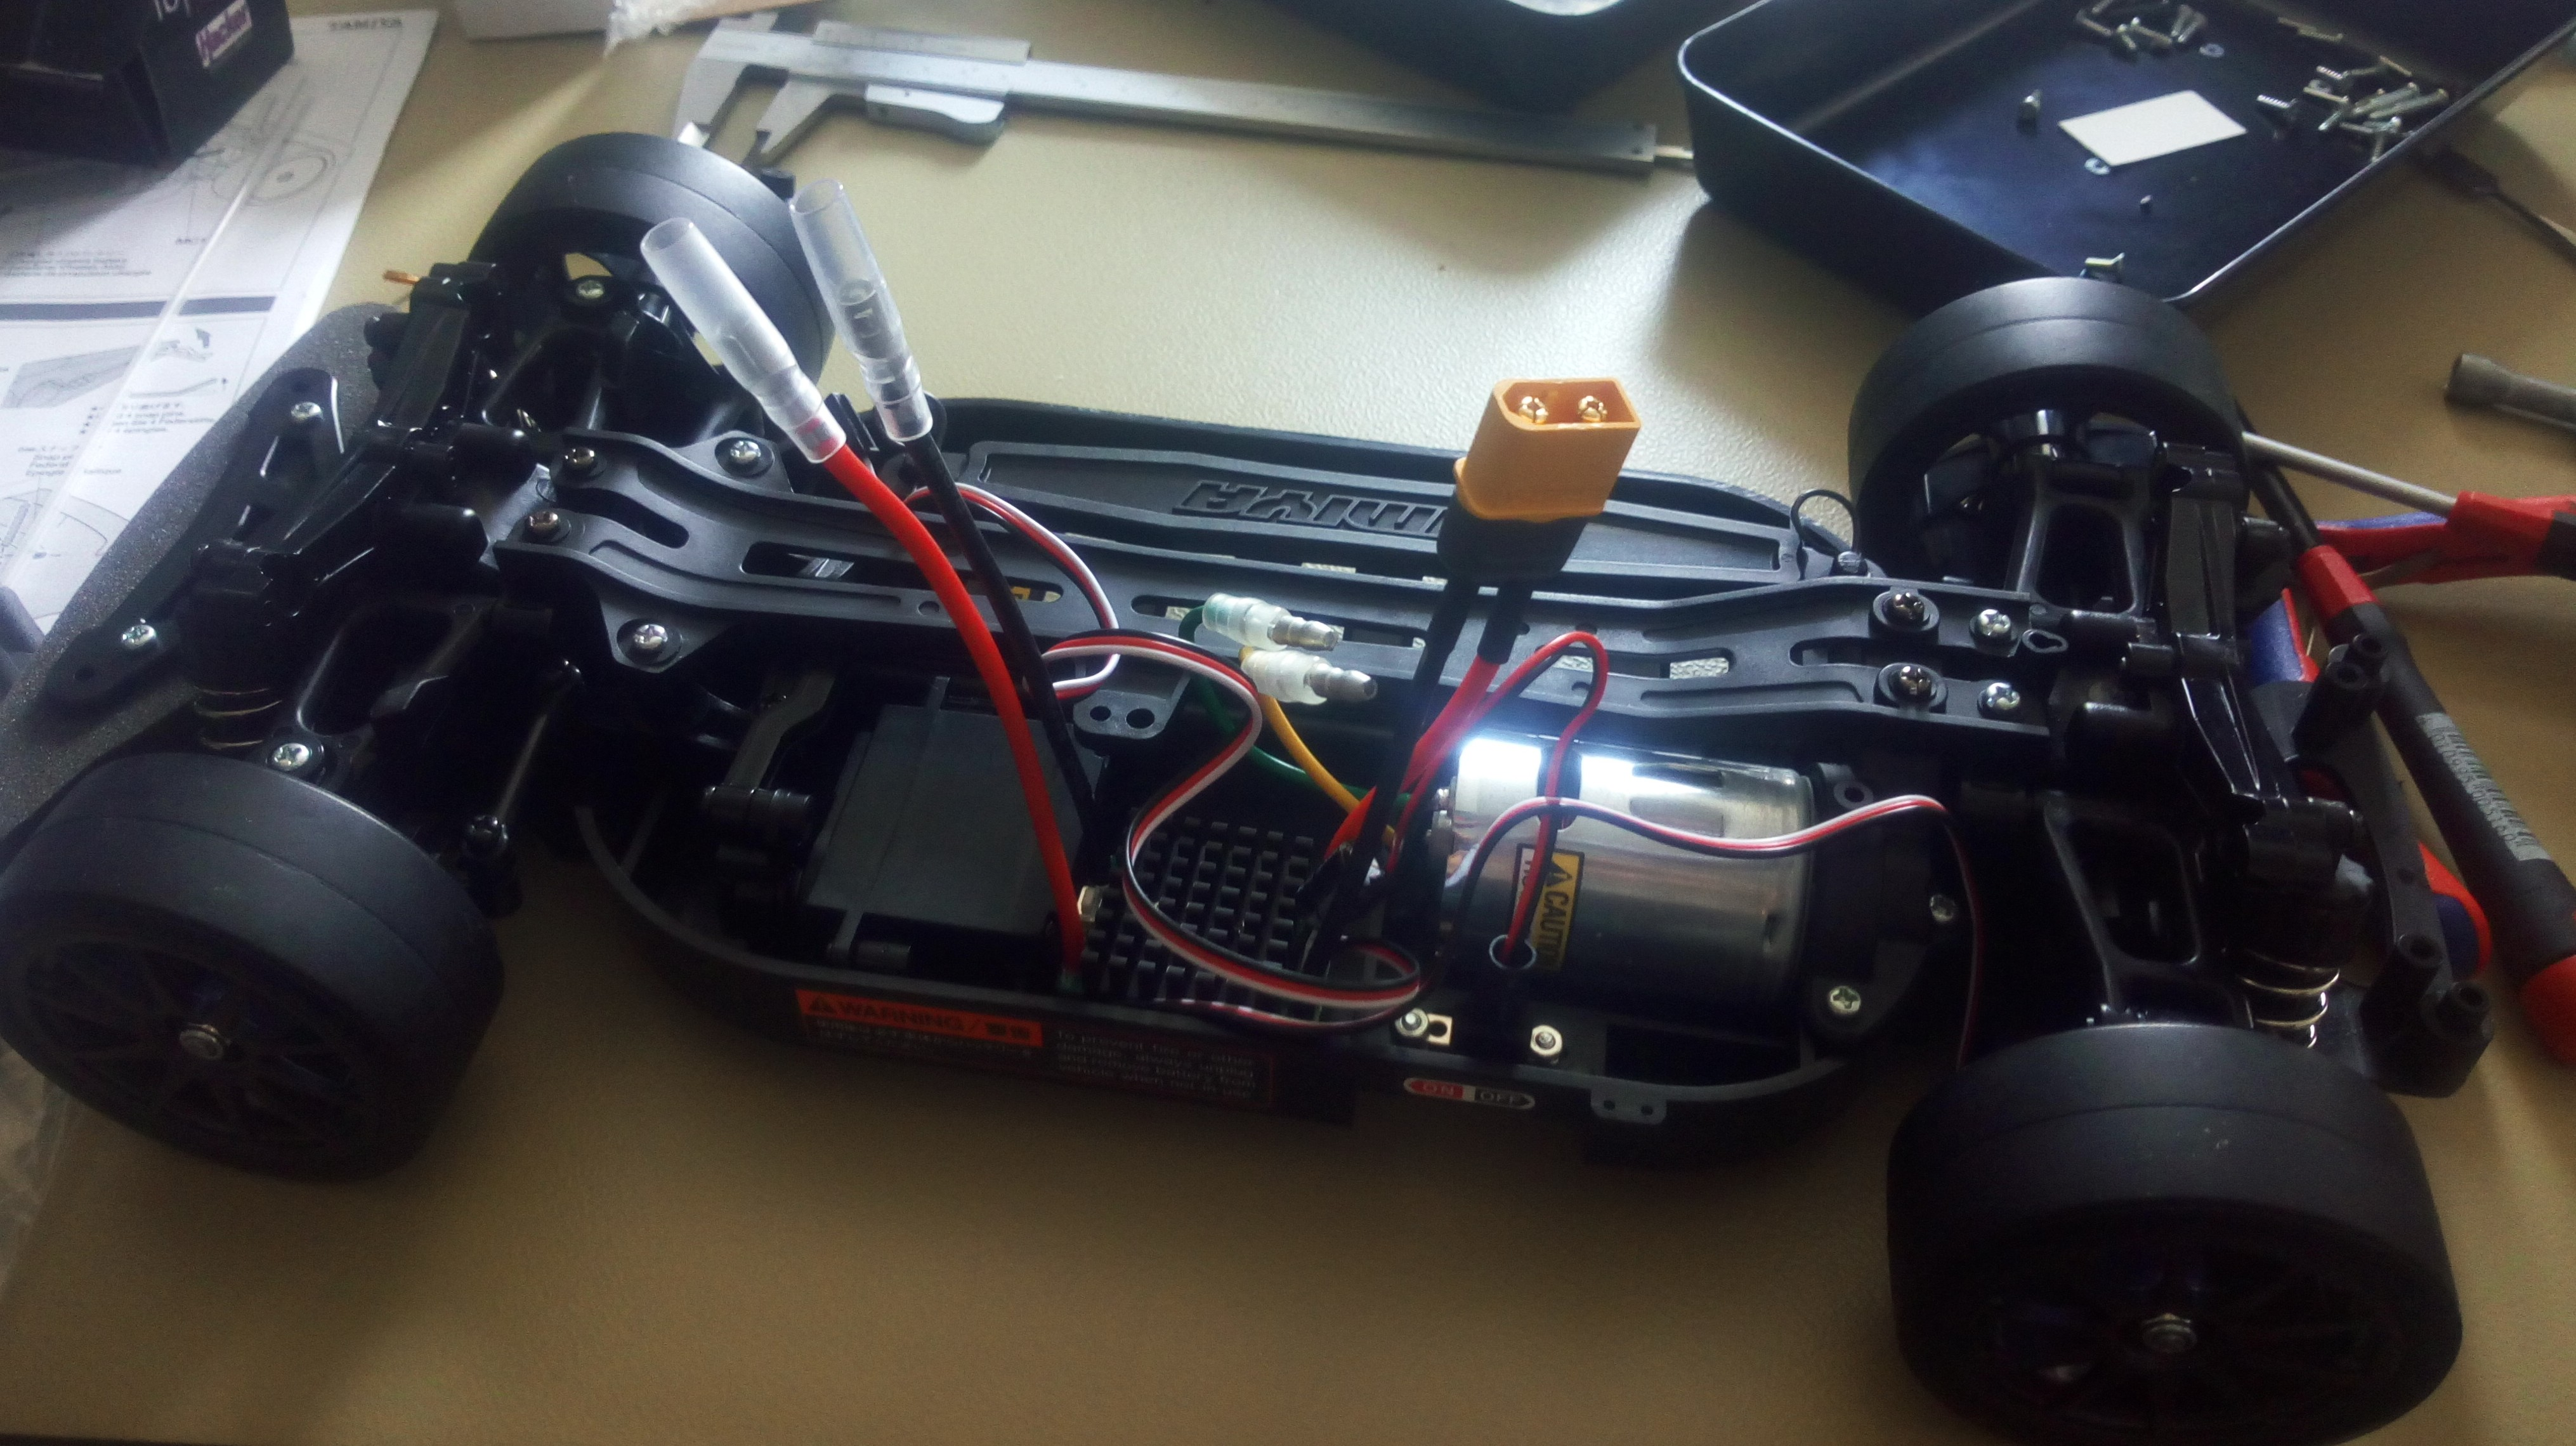
\includegraphics{img/car_body.jpg}}
\caption{Example of a figure caption.}
\label{fig}
\end{figure}
\end{comment}


%\section*{Acknowledgment}
% wollen wir unseren profs danken, weil mehr GPU und RAM? 

% wissenschaftliche zitate gehen so \cite{b1}. 


%Francis X. Govers - Artificial Intelligence for Robotics-Packt Publishing (2018).pdf
\begin{thebibliography}{00}
\bibitem{b1}Francis X. Govers , ` Artificial Intelligence for Robotics,''Packt Publishing ,2018

\end{thebibliography}


\end{document}
